Ve spolupráci s Jakubem Šístkem byly dokončeny práce na využití jeho 
paralelního řešiče implementujícího víceúrovňovou metodu BDDC. Práce zahrnovaly 
jak úpravy na straně Flow123d tak na straně knihovny. Aplikace metody BDDC na 
úlohy proudění s kombinacemi prvků různé dimenze je originální. Náročné bylo 
zejména zvládnutí velkých rozdílů ve vodivostech na rozhraních sub-struktur 
jednotlivých procesorů. Velké rozdíly se mohou objevit, pokud je rozhraní mezi 
prvky různé dimenze, kde může docházet k velkým skokům vodivosti na hranici 
rozhraní. Pro zvládnutí této heterogenity ve vodivosti bylo navrženy a 
otestovány tři metody vážení tlaků na rozhraních. Uvažujme bod $X$ na rozhraní 
sub-struktur $s=1,\dots,n$. Hodnota tlaku $p$ v tomto bodě je rovna váženému 
průměru tlaků $p_s$ na jednotlivých sub-strukturách, 
\[
    p = \sum_{s=1}^n p_s. 
\]

Standardní volba vah $w_s=1/n$ (aritmetický průměr) není vhodná pro heterogenní 
problémy. Pokud jsou materiálové parametry (v našem případě vodivost a 
rozevření puklin) výrazně rozdílné na jednotlivých sub-strukturách, používá se 
$\rho$-škálování:
\[
    w_s=\frac{\rho_s}{\sum_{s=1}^n \rho_s}.
\]
To ovšem předpokládá konstantní materiálové charakteristiky na jednotlivých 
sub-strukturách v našem případě $\rho_s=\frac{d}{\text{tr}(\tn K^{-1})}$, 
kde $d$ dimenze elementu a $\tn K$ je tenzor 
hydraulické vodivosti na elementu sub-struktury přiléhající k $X$. Kombinace 2D 
a 3D elementů však může vést k oscilacím, pokud se 
hodnoty $\rho_s$ výrazně mění podél rozhraní. Proto jsme navrhli upravené 
{\emph diagonální škálování}
\[
    \rho_s=C^s_{jj} + \frac{1}{A^s_{kk}},
\]
kde používáme přímo hodnoty z 
asemblované matice, $C^s_{jj}$ je diagonální hodnota z matice komunikace mezi 
dimenzemi. Ta je nenulová pouze v případě, že rozhraní odděluje elementy různé 
dimenze. Hodnota $A^s_{kk}$ je diagonální prvek z lokální matice elementu 
přiléhajícímu k rozhraní, chová se podobně jako $\tn K^{-1}$, ale zahrnuje i 
vliv geometrie. 




Tabulka \ref{tab:tunnel_averaging} demonstruje porovnání 
jednotlivých metod vážení, aritmetické vážení dává špatné výsledky i pro malý 
počet procesorů a někdy naprosto selhává (N=128, 1024), $\rho$-škálování dává 
většinou uspokojivé výsledky, ale selhává ve stejných případech jako aritmetické 
vážení. Jde o ty případy, kdy rozhraní sub-struktur leží 
mezi dimenzemi. Toto dělení je prováděno softwarem METIS a výskyt těchto 
patologických případů lze sice vhodným nastavením snížit, ale ne zcela vyloučit 
a to zejména pro větší počet sub-struktur. Poslední navržené škálování  však 
dobře funguje i s problematickým rozdělením. To demonstruje poslední sloupeček 
tabulky, kde
počet iterací ani číslo podmíněnosti příliš neroste s počtem sub-struktur.

\begin{table}[t]
\begin{center}
\begin{tabular}
[c]{|cc|ccc|cc|cc|cc|}\hline
\multirow{2}{*}{$N$} & \multirow{2}{*}{$n/N$} &
\multirow{2}{*}{$n_{\Gamma}$} & \multirow{2}{*}{$n_f$} &
\multirow{2}{*}{$n_c$} & \multicolumn{2}{c|}{aritmetický průměr} 
&
\multicolumn{2}{c|}{$\rho$-škálování} & \multicolumn{2}{c|}{diagonální 
škálování}\\
&  &  &  &  & its. & cond. & its. & cond. & its. & cond.\\\hline
32 & 245k & 20k & 106 & 322 & 637 & 9811.7 & 110 & 1467.8 & 112 & 1514.1\\
64 & 123k & 28k & 192 & 597 & 618 & 10254.1 & 62 & 115.1 & 63 & 117.7\\
128 & 61k & 45k & 413 & 1293 & 2834 & 1.0e+11 & 206 & 401641.4 & 75 & 194.4\\
256 & 31k & 72k & 902 & 2791 & 799 & 11172.9 & 117 & 512.9 & 119 & 526.7\\
512 & 15k & 110k & 2009 & 6347 & 883 & 15449.6 & 136 & 1160.1 & 137 & 1143.4\\
1024 & 8k & 155k & 4575 & 14725 & n/a & 2.5e+10 & 504 & 99023.6 & 173 &
897.0\\\hline
\end{tabular}
\end{center}
\caption{\label{tab:tunnel_averaging}
Vliv druhu vážení na počet iterací a odhad podmíněnosti matice.
\emph{tunel Bedřichov}, 2D a 3D elementy, 7.8 miliónů neznámých}
\end{table}

\begin{figure}[h]
\begin{center}
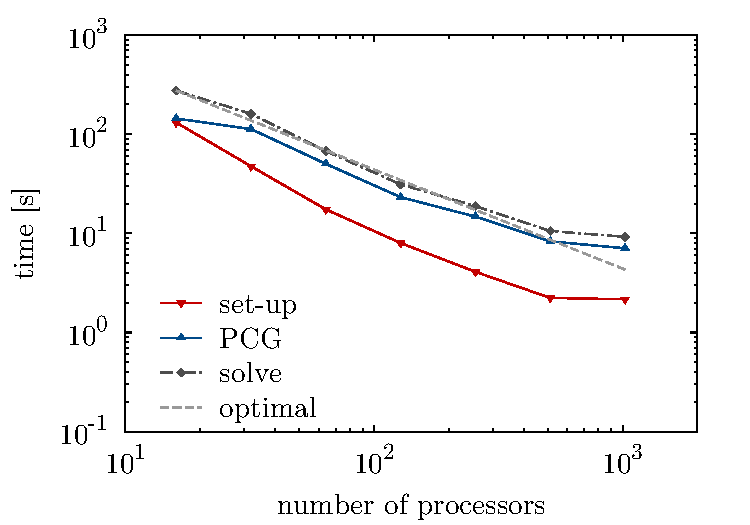
\includegraphics[width=0.48\textwidth]{timing_melechov_large} 
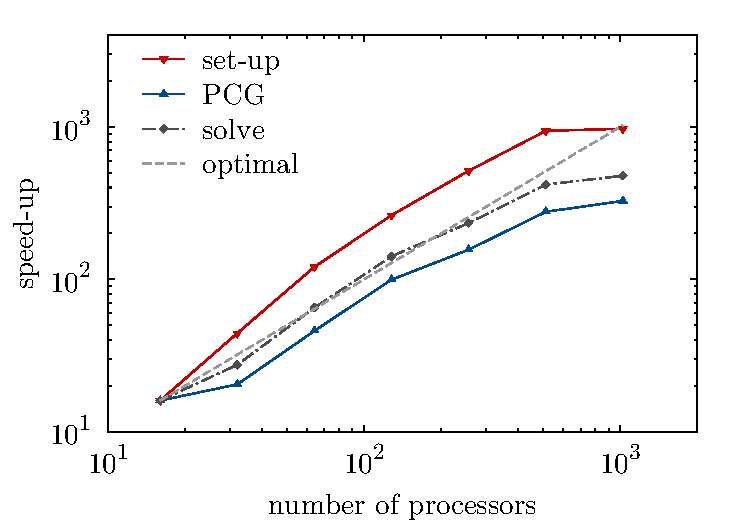
\includegraphics[width=0.48\textwidth]{speedup_melechov_large}
\end{center}
\caption{\label{fig:timing_Melechov_large}
Strong scaling test for the problem of the \emph{Melechov locality}
containing 2D and 3D elements and 15M unknowns, computational time (left) and
speed-up (right) separately for set-up and PCG phases, and their sum (solve).}
\end{figure}

Ve druhé polovině roku 2013 byl řešič využívající knihovnu BDDCML začleněn do 
hlavní produkční větve a součástí verze 1.8.0. S využitím knihovny BDDCML bylo 
dosaženo velmi dobré silné škálovatelnosti při řešení velkých reálných úloh 
(miliony elementů) při využití až tisíce výpočetních jader, viz Obrázek~2. 
Výsledky byly shrnuty v článku \cite{SistekBDDC} zaslaného k recenzi.
